\documentclass[10pt,aspectratio=169]{beamer}

%================================================
% Theme
%================================================
\usetheme[numbering=fraction,progressbar=frametitle]{metropolis}

%================================================
% Packages
%================================================
\usepackage{amsmath,amssymb}
\usepackage{booktabs}
\usepackage{xcolor}
\usepackage{listings}
\usepackage{tikz}
\usepackage[useregional]{datetime2}
\usetikzlibrary{positioning,arrows.meta,shapes.geometric}

%================================================
% Metadata macros
%================================================
\newcommand{\CourseName}{Theory of Computation}
\newcommand{\LectureTitle}{Lecture 2: Languages, Problems, and the Idea of Computation}
\newcommand{\LastCompiledTime}{\DTMnow}

\title{\CourseName}
\subtitle{\LectureTitle}
\author{Sheikh Azizul Hakim\\Lecturer, Department of CSE, BUET}
\date{Last compiled: \LastCompiledTime}

%================================================
% Colors and styles
%================================================
\definecolor{tocblue}{HTML}{2457C5}
\definecolor{tocgreen}{HTML}{0B7A75}
\definecolor{tocorange}{HTML}{D9822B}
\definecolor{tocpurple}{HTML}{6F42C1}
\definecolor{softgray}{HTML}{F3F4F6}

\setbeamercolor{alerted text}{fg=tocblue}

%================================================
% Code style
%================================================
\lstdefinestyle{code}{
  basicstyle=\ttfamily\small,
  backgroundcolor=\color{black!4},
  frame=single,
  rulecolor=\color{black!20},
  columns=fullflexible,
  keepspaces=true,
  showstringspaces=false
}
\lstset{style=code}

%================================================
% Helper macros
%================================================
\newcommand{\term}[1]{\textcolor{tocblue}{\textbf{#1}}}
\newcommand{\keyidea}[1]{\begin{center}\alert{\textbf{#1}}\end{center}}
\newcommand{\mathbox}[1]{%
\begin{center}
\colorbox{black!4}{\parbox{0.86\textwidth}{\centering #1}}
\end{center}}

%================================================
\begin{document}

%------------------------------------------------
\maketitle

%------------------------------------------------
\begin{frame}[standout]
Everything that a computer processes can be represented as strings.

\vspace{1em}

Everything.
\end{frame}

%------------------------------------------------
\begin{frame}[fragile]{Is This Data?}
\begin{columns}[T]
\column{0.48\textwidth}
\begin{lstlisting}
42
01101010
if (x > 5)
\end{lstlisting}

\column{0.48\textwidth}
\begin{lstlisting}
ATTGCCGA
<emoji>
Write a poem.
\end{lstlisting}
\end{columns}

\vspace{1em}

\pause
\begin{center}
What do these have in common?
\end{center}

\pause
\keyidea{They are finite sequences of symbols.}
\end{frame}

%------------------------------------------------
\begin{frame}{Everything Is Strings}
\begin{center}
\begin{tabular}{ll}
\toprule
\textbf{Object} & \textbf{String representation} \\
\midrule
Integer & \texttt{12345} \\
DNA sequence & \texttt{ACTGACTG} \\
Program & \texttt{if (x > 5) \{ ... \}} \\
Image & JPEG/PNG bit stream \\
Audio & MP3/WAV bit stream \\
Prompt & \texttt{``Write a poem.''} \\
\bottomrule
\end{tabular}
\end{center}

\vspace{1em}

\pause
\begin{center}
\textbf{Data} $\longrightarrow$ \textbf{Strings}
\end{center}
\end{frame}

%------------------------------------------------
\begin{frame}{Alphabet}
An \term{alphabet} is a finite nonempty set of symbols.

\vspace{1.2em}

\pause
Examples:

\begin{align*}
\Sigma_1 &= \{0,1\}, \\
\Sigma_2 &= \{a,b,c,\ldots,z\}, \\
\Sigma_3 &= \{A,C,G,T\}.
\end{align*}

\pause
\vspace{0.5em}

In computation, we choose an alphabet according to the kind of objects we want to encode.
\end{frame}

%------------------------------------------------
\begin{frame}{Strings}
Over the alphabet
\[
\Sigma = \{0,1\},
\]
examples of strings are:

\mathbox{$\varepsilon,\quad 0,\quad 1,\quad 01,\quad 1011,\quad 111000$}

\pause
\vspace{0.5em}

The \term{length} of a string is the number of symbols in it:
\[
|1011| = 4, \qquad |\varepsilon| = 0.
\]
\end{frame}

%------------------------------------------------
\begin{frame}{String Operations}
\textbf{Concatenation}
\[
01 \cdot 10 = 0110.
\]

\pause
\textbf{Power}
\[
0^2 = 00, \qquad (ab)^3 = ababab.
\]

\pause
\textbf{Reverse}
\[
(10110)^R = 01101.
\]

\vspace{0.5em}
\pause
\begin{center}
Strings are simple objects, but they can encode almost anything.
\end{center}
\end{frame}

%------------------------------------------------
\begin{frame}{All Possible Strings}
For an alphabet $\Sigma$, the set of all finite strings over $\Sigma$ is written:
\[
\Sigma^*.
\]

\pause
For $\Sigma=\{0,1\}$,
\[
\Sigma^* = \{\varepsilon,0,1,00,01,10,11,000,\ldots\}.
\]

\pause
\vspace{0.5em}
\begin{center}
Is $\Sigma^*$ finite or infinite?
\end{center}
\end{frame}

%------------------------------------------------
\begin{frame}{What Is a Language?}
A \term{language} is a set of strings.

\vspace{1.2em}

\pause
If $\Sigma = \{0,1\}$, then each of the following is a language:

\begin{align*}
L_1 &= \{0, 10, 111\}, \\
L_2 &= \{w \in \Sigma^* : w \text{ contains an even number of } 1\text{s}\}, \\
L_3 &= \Sigma^*, \\
L_4 &= \emptyset.
\end{align*}

\pause
\keyidea{A language separates YES strings from NO strings.}
\end{frame}

%------------------------------------------------
\begin{frame}{Computational Problems}
Consider these questions:

\vspace{0.5em}

\begin{itemize}
\item Is \texttt{100101} divisible by 3?
\item Is \texttt{(()())} balanced?
\item Is this Python program syntactically valid?
\item Is this Boolean formula satisfiable?
\end{itemize}

\pause
\vspace{1em}

\begin{center}
What do these problems have in common?
\end{center}

\pause
\keyidea{Each input has a YES or NO answer.}
\end{frame}

%------------------------------------------------
\begin{frame}{The Central Idea}
\begin{center}
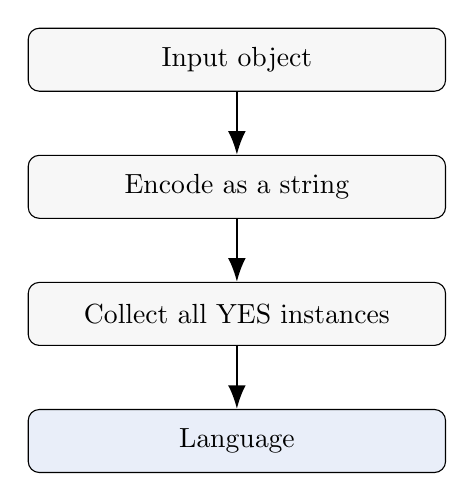
\begin{tikzpicture}[
    node distance=0.8cm,
    box/.style={draw, rounded corners, minimum width=5.3cm, minimum height=0.8cm, align=center, fill=black!3},
    arrow/.style={-{Latex[length=3mm]}, thick}
]

\node[box] (input) {Input object};
\node[box, below=of input] (encode) {Encode as a string};
\node[box, below=of encode] (yes) {Collect all YES instances};
\node[box, below=of yes, fill=tocblue!10] (lang) {Language};

\draw[arrow] (input) -- (encode);
\draw[arrow] (encode) -- (yes);
\draw[arrow] (yes) -- (lang);

\end{tikzpicture}
\end{center}

\pause
\vspace{0.6em}

\begin{center}
A computational problem becomes a language.
\end{center}
\end{frame}

%------------------------------------------------
\begin{frame}{Example: Even Number of 1's}
Define:
\[
L_{\mathrm{even}} = \{ w \in \{0,1\}^* : w \text{ contains an even number of } 1\text{s} \}.
\]

\pause
\begin{columns}[T]
\column{0.48\textwidth}
\textbf{In the language}
\[
\varepsilon,\quad 00,\quad 11,\quad 1010,\quad 010101
\]

\column{0.48\textwidth}
\textbf{Not in the language}
\[
1,\quad 111,\quad 101,\quad 0001000
\]
\end{columns}

\pause
\vspace{0.6em}
\begin{center}
Soon we will build a tiny machine that recognizes this language.
\end{center}
\end{frame}

%------------------------------------------------
\begin{frame}{Example: Palindromes}
A palindrome reads the same forward and backward.

\pause
\[
\mathrm{PAL} = \{ w \in \{0,1\}^* : w = w^R \}.
\]

\pause
\begin{columns}[T]
\column{0.48\textwidth}
\textbf{Examples}
\[
0,\quad 1,\quad 0110,\quad 1001,\quad 01010
\]

\column{0.48\textwidth}
\textbf{Non-examples}
\[
01,\quad 110,\quad 0101,\quad 10010
\]
\end{columns}

\pause
\vspace{0.5em}
\begin{center}
This language requires more memory than finite automata have.
\end{center}
\end{frame}

%------------------------------------------------
\begin{frame}[fragile]{Example: Valid JSON}
An LLM may be asked:

\begin{lstlisting}
Generate a valid JSON object.
\end{lstlisting}

\pause
Valid JSON:
\begin{lstlisting}
{
  "name": "Aziz",
  "courses": ["CSE", "EEE"]
}
\end{lstlisting}

\pause
The corresponding language is:
\[
\mathrm{JSON} = \{x : x \text{ is a syntactically valid JSON string}\}.
\]

\pause
\keyidea{Structured generation is language generation.}
\end{frame}

%------------------------------------------------
\begin{frame}[fragile]{Example: Valid Python Programs}
Question:

\begin{center}
What language is recognized by Python's parser?
\end{center}

\pause
\[
\mathrm{PYTHON} = \{x : x \text{ is a syntactically valid Python program}\}.
\]

\pause
\begin{lstlisting}
def square(x):
    return x*x
\end{lstlisting}

\pause
\begin{center}
Programming languages are literally languages.
\end{center}
\end{frame}

%------------------------------------------------
\begin{frame}{Example: SAT}
A Boolean formula is \term{satisfiable} if some assignment of truth values makes it true.

\pause
\[
\mathrm{SAT} = \{\varphi : \varphi \text{ is satisfiable}\}.
\]

\pause
\begin{columns}[T]
\column{0.48\textwidth}
\textbf{YES instance}
\[
(x \lor y) \land (\neg x \lor z)
\]

\column{0.48\textwidth}
\textbf{NO instance}
\[
x \land \neg x
\]
\end{columns}

\pause
\vspace{1em}
\begin{center}
SAT is one of the most important languages in computer science.
\end{center}
\end{frame}

%------------------------------------------------
\begin{frame}{Why Languages?}
Without a common abstraction, these look unrelated:

\vspace{0.7em}

\begin{center}
\begin{tabular}{ccccc}
sorting & images & graphs & AI prompts & DNA
\end{tabular}
\end{center}

\pause
\vspace{1.5em}

With languages:

\begin{center}
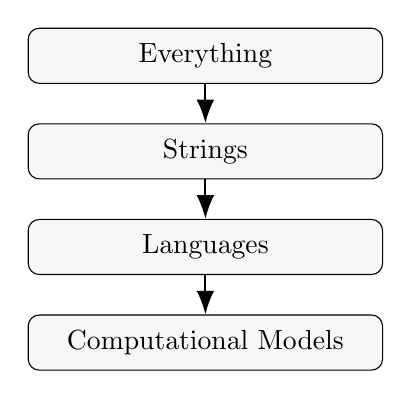
\begin{tikzpicture}[
    node distance=0.5cm,
    box/.style={draw, rounded corners, minimum width=4.5cm, minimum height=0.7cm, align=center, fill=black!3},
    arrow/.style={-{Latex[length=3mm]}, thick}
]
\node[box] (everything) {Everything};
\node[box, below=of everything] (strings) {Strings};
\node[box, below=of strings] (languages) {Languages};
\node[box, below=of languages] (models) {Computational Models};
\draw[arrow] (everything) -- (strings);
\draw[arrow] (strings) -- (languages);
\draw[arrow] (languages) -- (models);
\end{tikzpicture}
\end{center}


\end{frame}

%------------------------------------------------
\begin{frame}{Which Machines Recognize Which Languages?}
\begin{center}
\begin{tabular}{lll}
\toprule
\textbf{Machine model} & \textbf{Memory idea} & \textbf{Language class} \\
\midrule
Finite Automata & finite memory & Regular Languages \\
Pushdown Automata & one stack & Context-Free Languages \\
Turing Machines & unbounded memory & Computable Languages \\
Efficient Algorithms & bounded resources & Complexity Classes \\
\bottomrule
\end{tabular}
\end{center}

\pause
\vspace{1.5em}

\begin{center}
This is the roadmap of the course.
\end{center}
\end{frame}

%------------------------------------------------
\begin{frame}{Mini Assignment}
Define each of the following as a language.

\begin{enumerate}
    \item Valid BUET student IDs.
    \item Valid email addresses.
    \item Valid JSON objects.
    \item Binary strings representing numbers divisible by 5.
\end{enumerate}

\end{frame}

%------------------------------------------------
\begin{frame}[standout]
Everything can be encoded as strings.

\vspace{1em}

Every computational problem can be viewed as a language.

\vspace{1em}

Theory of Computation asks:

\vspace{0.5em}

\textit{Which machines can recognize which languages?}
\end{frame}

%================================================
\end{document}
